\documentclass[../poliXuniversity_hospital_(USP)_report.tex]{subfiles}

\begin{document}

\chapter{Software Golgi}

\section{Algorítimo de movimentação}

\subsection{Máquina de estados}

Usando o conceito de máquina de estados podemos controlar nossa maquina e garantir o sucesso de cada etapa.

ESTADOS:

STAND-BY: Aguarda receber via Comunicação Serial um index de 0 a 95(cabides) que sera seu alvo. Assim que o index é recebido o estado é alterado para GOING

GOING: Ativa o algoritimo de controle e faz com que o apanhador vá em direção ao seu alvo. Quando ambos eixos X e Z estão no alvo(+-2mm) o estado é alterado para GETING-MEDICINE. 

GETING-MEDICINE: Após chegar a posição desejada, ativa a captura do rémedio. Que consiste na extensão e contrção do atuador com a bomba de vácuo ligada, usando o sensor de pressão é possivel identificar a captura ou não do envelope. Caso o sensor indique falha na captura, a rotina de extensão e contração se repete, se bem sucedido o estado é alterado para DROPING-MEDICINE.

DROPING-MEDICINE:Após a certificação da captura, a estrutura retorna ao cesto onde o remédio deve ser depositado. Com a finalização dessa rotina o estado é alterado para STAND-BY.
\begin{figure}[h]
\centering
    \caption{Máquina de estados Loop ESP-32}
    \centering % para centralizarmos a figura
    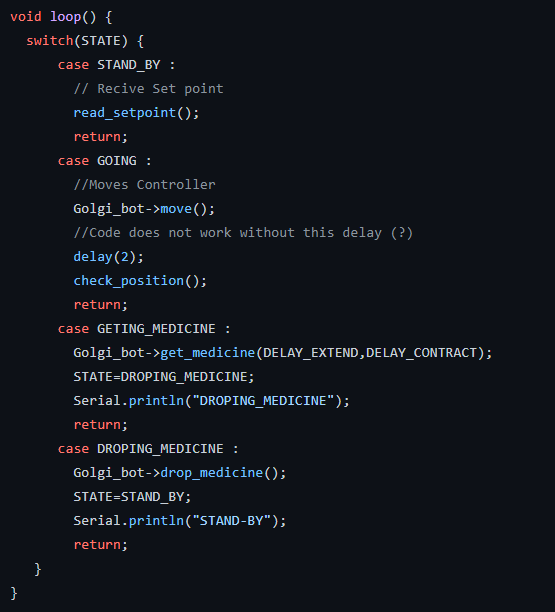
\includegraphics[width=5cm]{images/maquina_de_estados.png}
    \caption*{Fonte: Autor}
    \label{figura: Máquina de estados Loop ESP-32}
\end{figure}
\subsection{Controle PID}

Para o controle de posição do apanhador foram usados dois controladores PID, um em cada eixo de movimentação. O codigo foi desenvolvido em C++ para ser usado na função loop do ESP32. Foram desensolvidos bibliotecas orientadas objeto para realização de todos calculos e aquisição de dados de realimentação dos encoderes. Para a calibraão dos parametros não foi realizada o trabalho analitico de obtenção de equação da planta, apenas foi realizado o ajusto empirico das constantes proporcional, integratva e derivativa de tal forma a se obter a tolerancia proposta de 2mm.

\begin{figure}[h]
\centering
     \caption{Diagrama de blocos Controle em X}
        \centering % para centralizarmos a figura
        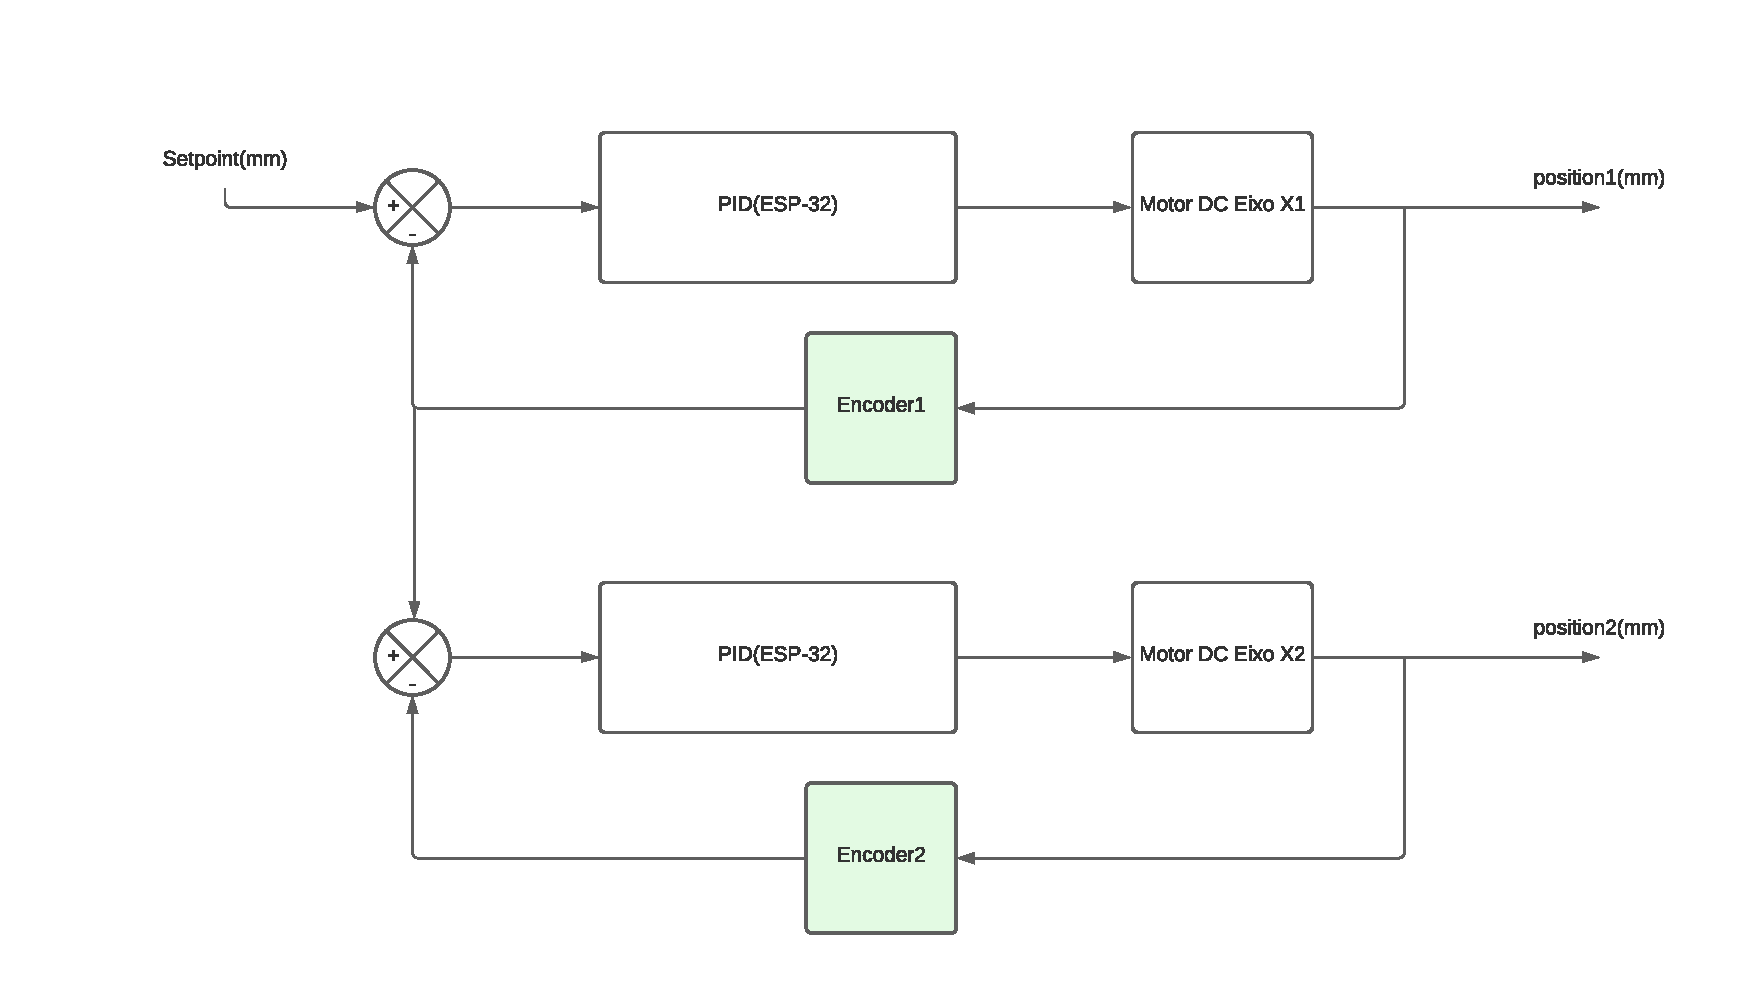
\includegraphics[width=10cm]{images/Diagrama de blocos X.pdf}
        \caption*{Fonte: Autor}
        \label{figura: Diagrama de blocos Controle em X}
\end{figure}

\begin{figure}[h]
\centering
    \caption{Diagrama de blocos Controle em Z}
        \centering % para centralizarmos a figura
        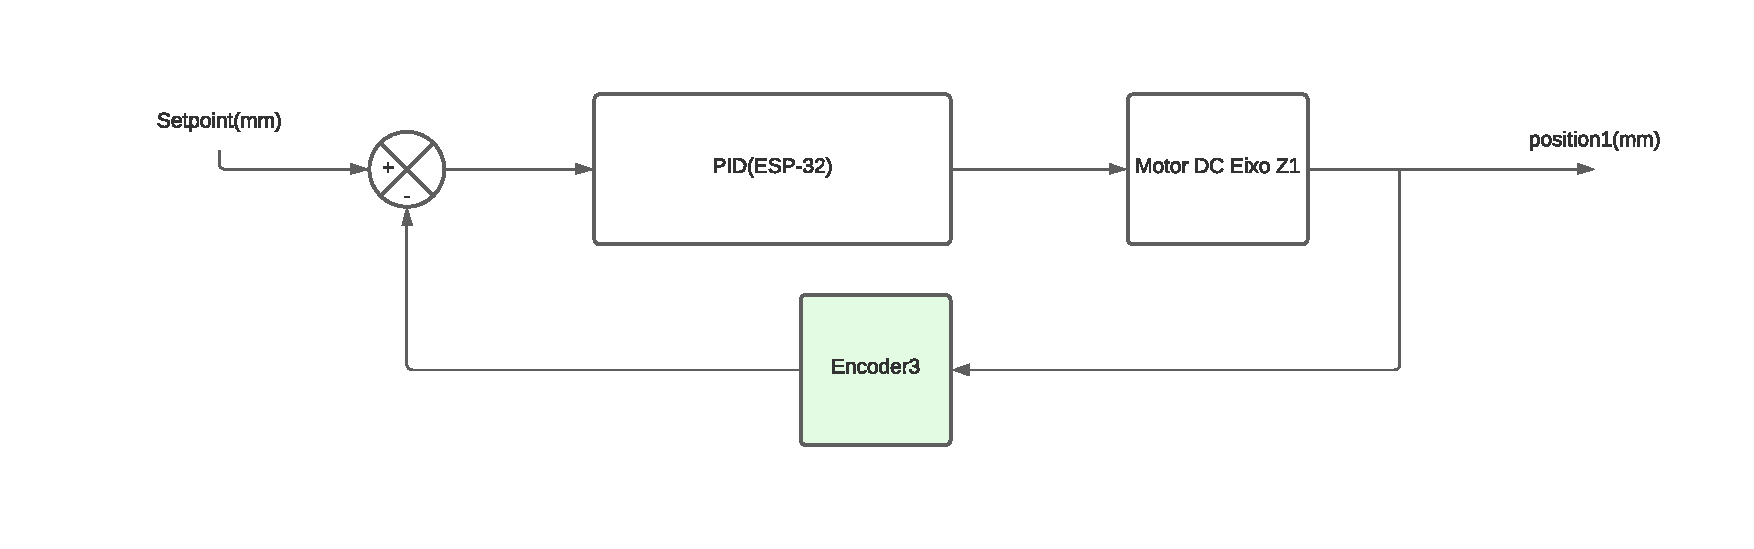
\includegraphics[width=10cm]{images/Diagrama de blocos Z.pdf}
        \caption*{Fonte: Autor}
        \label{figura: Diagrama de blocos Controle em Z}
\end{figure}


\section{Interface com usuários}

\subsection{Controle de estoque}
Para realizar o controle de estoque foi desenvolvido um sistema de registro dos farmacos a serem armazenados na maquina bem como o controle desses itens. Hosteado no microprocessador raspberry pi b+ o software desenvolvido em Python utiliza a biblioteca Kivy para interface gráfica. Atraves do sistema é possivel realizar a solicitação de retirada de remedio, recaregamendo da máquina, cadastro de pacientes e armazenamento de todas interações e seus respectivos responsáveis(funcionarios da farmácia)
\begin{figure}[h]
\centering
    \begin{minipage}{0.5\textwidth}
        \centering
        \caption{Kivy}
        \centering % para centralizarmos a figura
        
\includegraphics[width=6cm]{images/Kivy_logo.png}
        \caption*{Fonte: Kivy}
        \label{figura: Kivy}
        
    \end{minipage}\hfill
    \begin{minipage}{0.5\textwidth}
    
        \centering
        \caption{Sistema Golgi}
        \centering % para centralizarmos a figura
        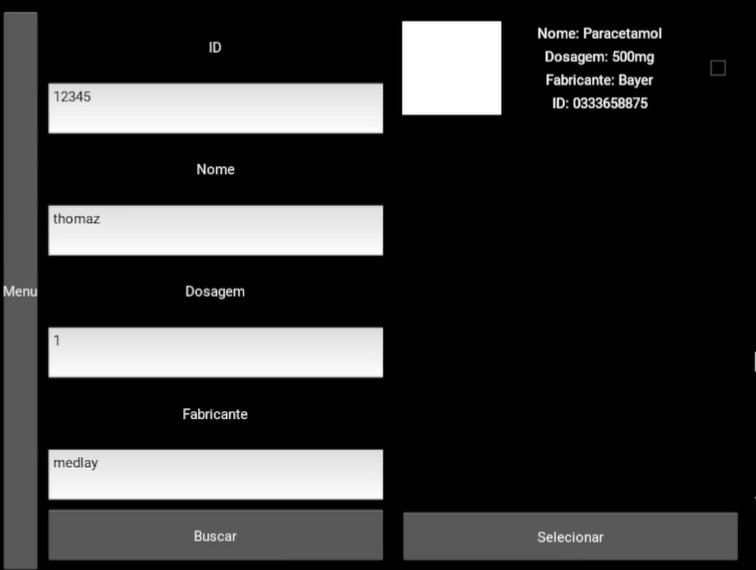
\includegraphics[width=6cm]{images/sistema_golgi.png}
        \caption*{Fonte: Autor}
        \label{figura: Sistema Golgi}
        
    \end{minipage}\hfill
\end{figure}

\subsection{Autenticação}

Buscando manter a segurança, foi implementado a indentificação por RFID e fechamento por trava solenoide como mecanismos de segurança. Apenas funcionários previamente cadastrados serão liberados com seu cracha USP e as travas solenoides e batentes garantem que as portas so se abram para os autenticados.
\begin{figure}[h]
\centering
    \begin{minipage}{0.5\textwidth}
        \centering
        \caption{Módulo RFID}
        \centering % para centralizarmos a figura
        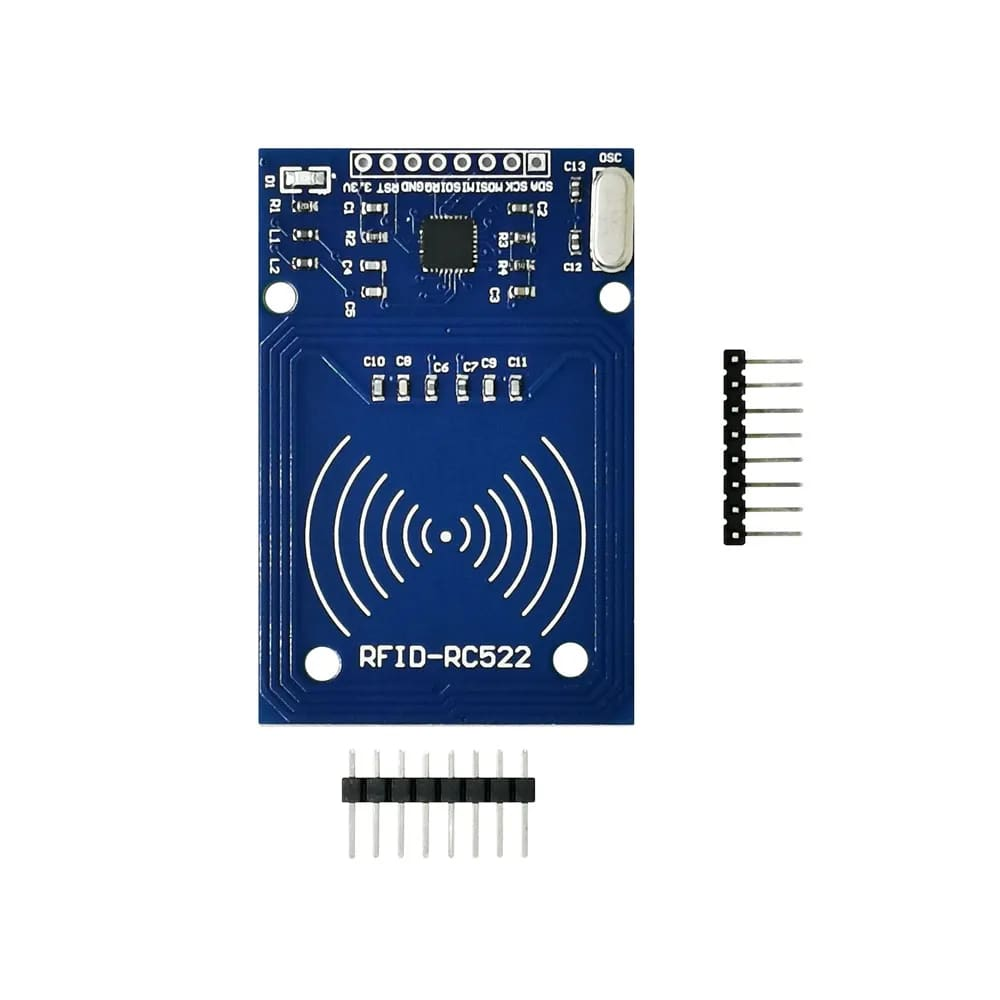
\includegraphics[width=7cm]{images/rfid.jpg}
        \caption*{Fonte: WJ componentes}
        \label{figura: Módulo RFID}
        
    \end{minipage}\hfill
    \begin{minipage}{0.5\textwidth}
    
        \centering
        \caption{Solenoide 12V}
        \centering % para centralizarmos a figura
        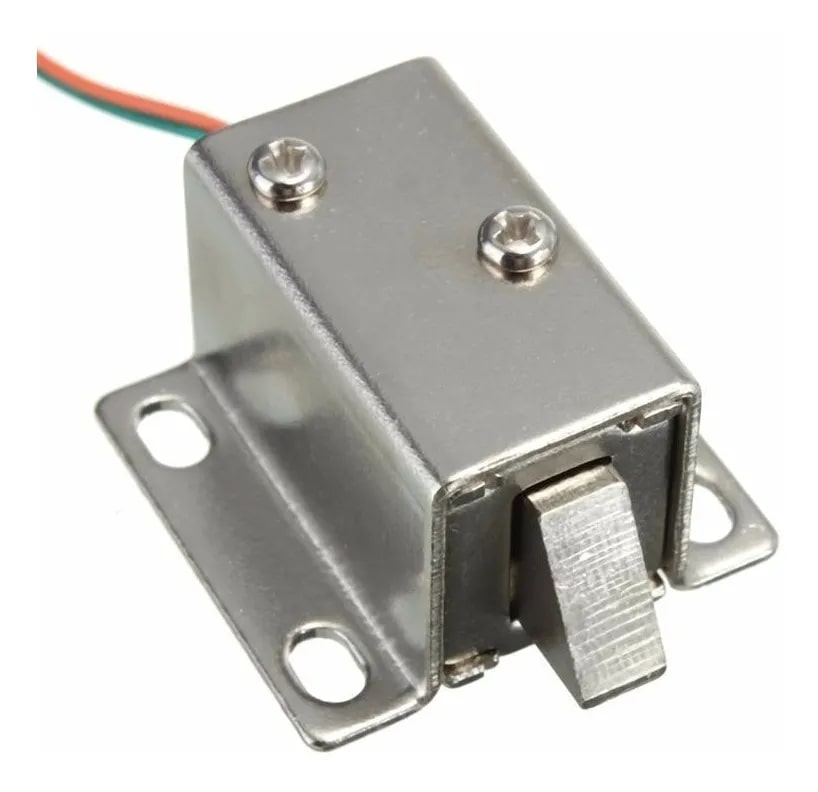
\includegraphics[width=7cm]{images/solenoide .jpg}
        \caption*{Fonte: Mercado Livre}
        \label{figura: Solenoide 12V}
        
    \end{minipage}\hfill
\end{figure}


\end{document}